\documentclass[../main/main.tex]{subfiles}

\begin{document}

\section{Testing with Pycharm} 

\subsection{Setting up the project}

A new Python 3.4 project was created in Pycharm. This turned out to be
very easy, so it is not necessary to revise the steps that I went
through. 

Afterwards, I created a module in the root directory called
\lstinline|bruch|. In this module I wrote the class \lstinline|Bruch|
by overriding all the necessary magic functions,
e.g. \lstinline|__add__()|, \lstinline|__isub__()|, that were used in
the given tests.

The tests were included in a separate directory called
\lstinline|test|. Afterwards, I created a run configuration that
executed all tests in the previously mentioned \lstinline|test|
directory. The configuration can be seen in Figure \ref{fig:edit}.

\begin{figure}[H]
  \centering
  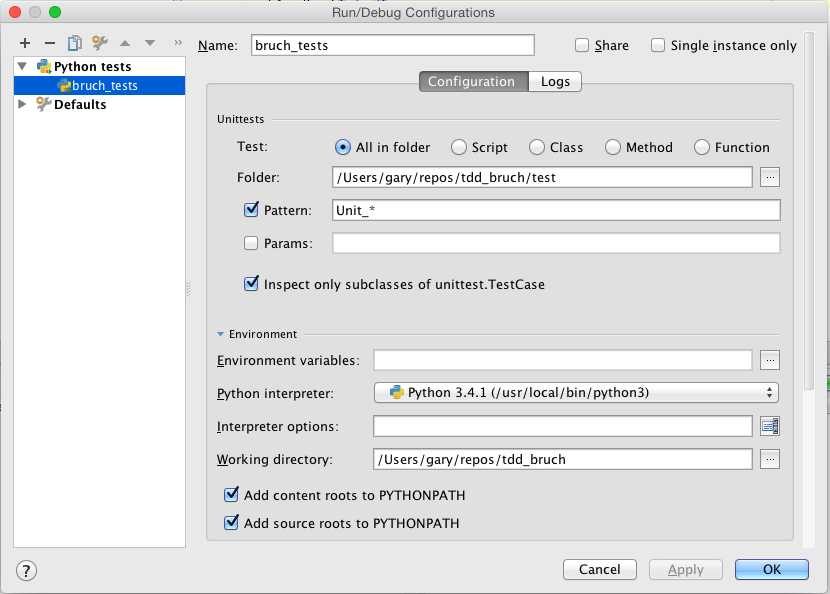
\includegraphics[width=0.7\linewidth]{../figures/edit_config.png}
  \caption{Edit configuration for tests}
  \label{fig:edit}
\end{figure}

A simple hit on the run button will execute all the tests
appropriately.

\subsection{Coverage Report (HTML)}

By selecting the \textit{Run with Coverage} option, one
can also generate a coverage report, which can take a while. 

An HTML report can be generated by first running the \textit{Run with
  Coverage} option, and subsequently selecting \textit{Tools/Generate
  Coverage Report}.

The report of this exercise, which are generated in HTML files, can be
found in the \textit{report/} directory, but can also be seen in
Figure \ref{fig:coverage}. 

\begin{figure}[H]
  \centering
  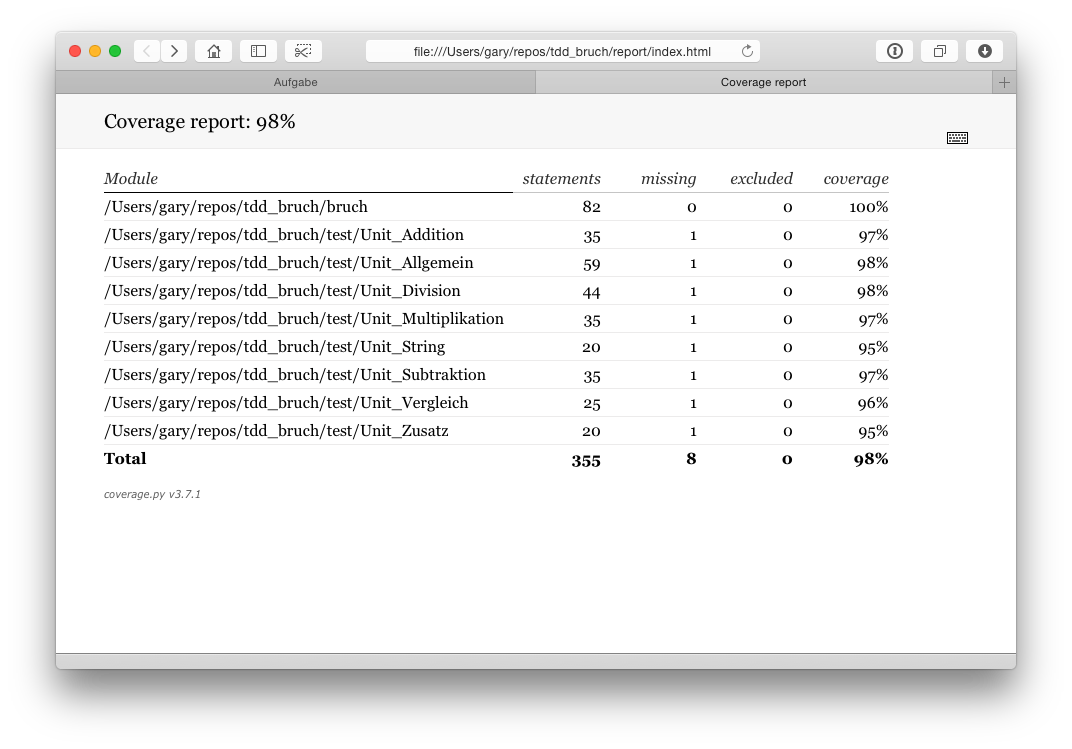
\includegraphics[width=\linewidth]{../figures/coverage_report.png}
  \caption{Coverage report}
  \label{fig:coverage}
\end{figure}

The fraction class was written such that it passed all test cases,
which was successful as we can see in Figure \ref{fig:unit}, which is
a screenshot from the test report generated by Pycharm. The report can be generated by clicking on the ``Export'' button in, as seen in \ref{fig:export}.

\begin{figure}[H]
  \centering
  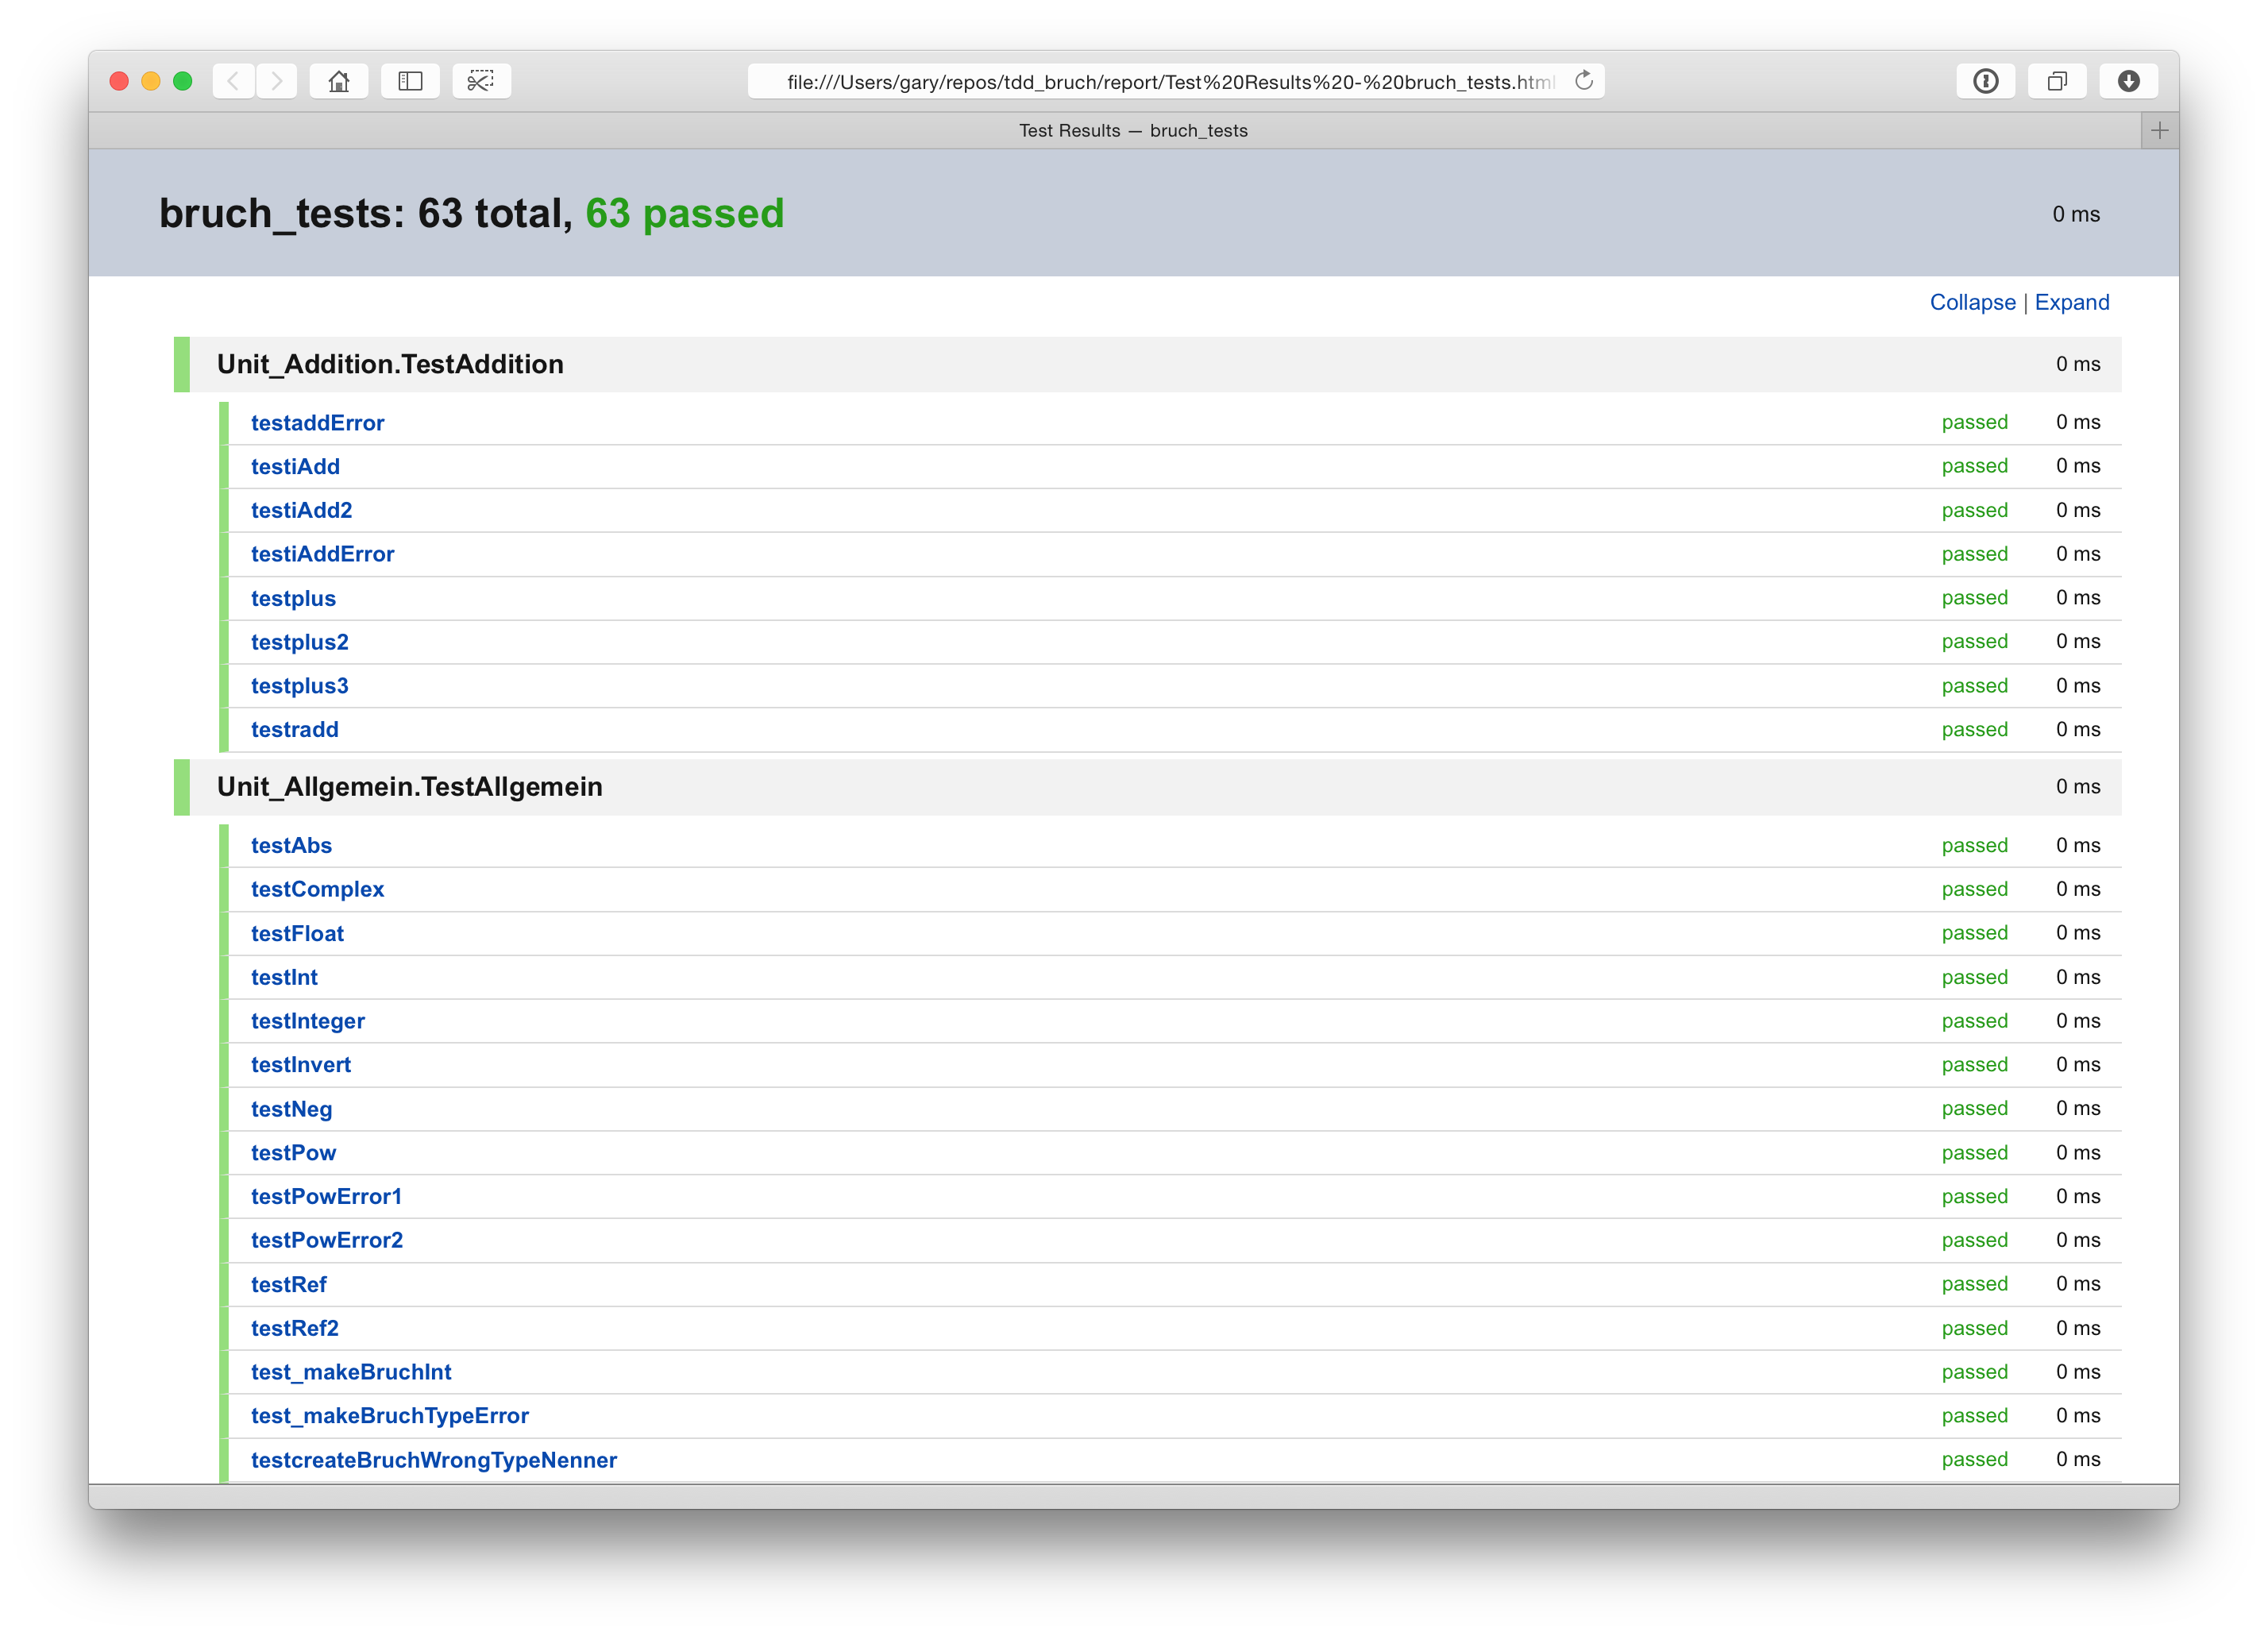
\includegraphics[width=0.7\linewidth]{../figures/unit_testing.png}
  \caption{Unit testing.}
  \label{fig:unit}
\end{figure}

\begin{figure}[H]
  \centering
  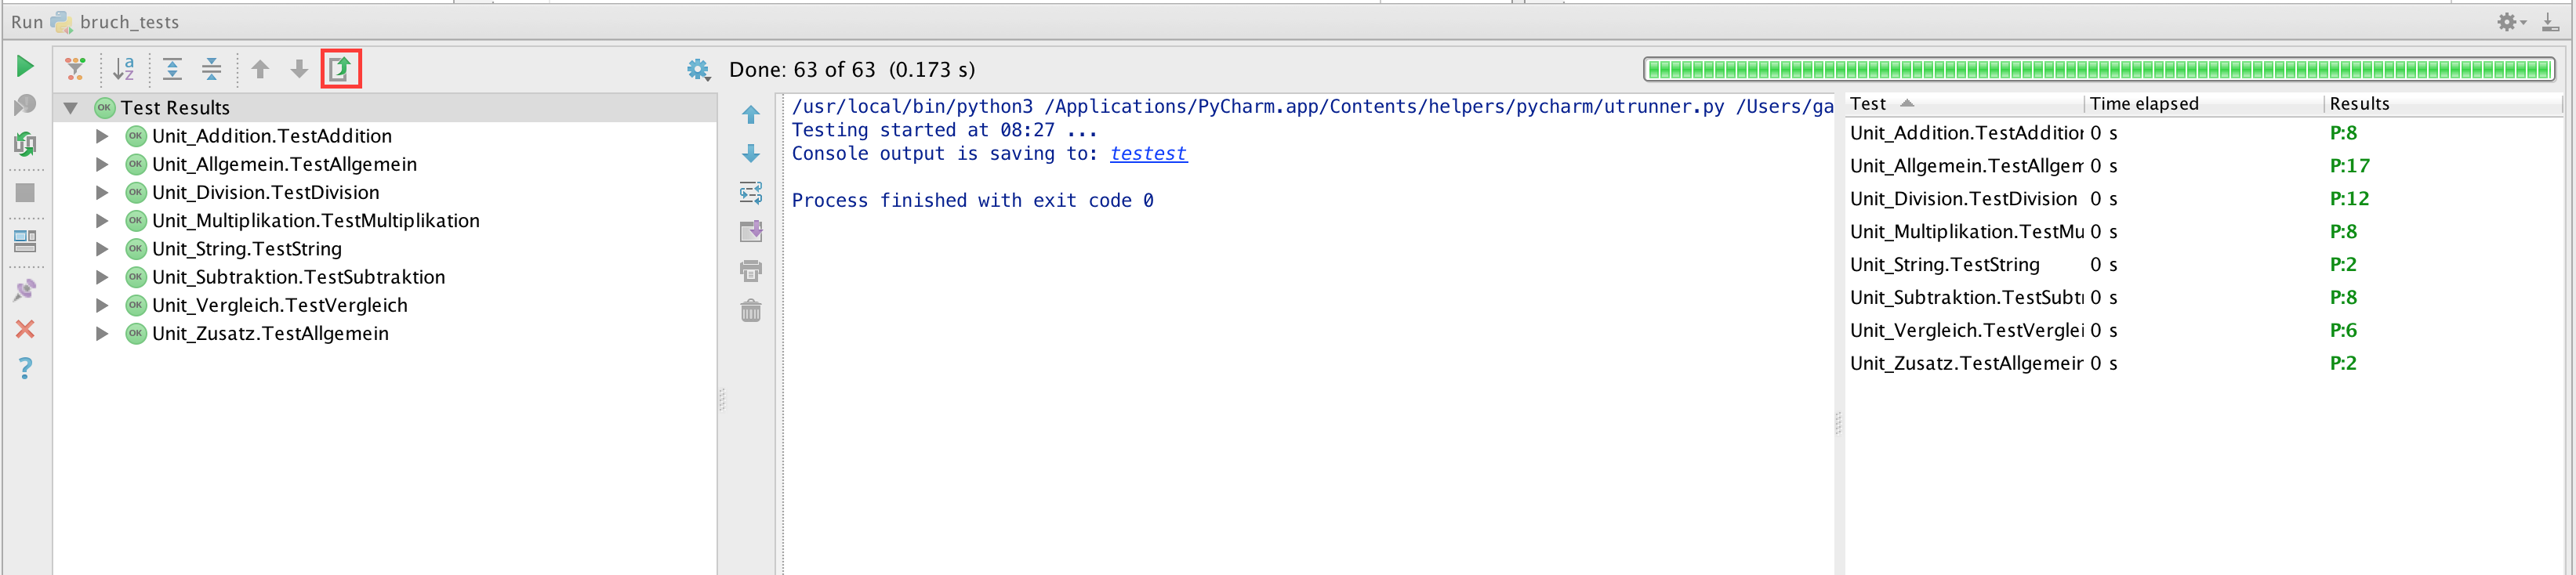
\includegraphics[width=0.8\linewidth]{../figures/export.png}
  \caption{Exporting the unit tests.}
  \label{fig:export}
\end{figure}


\end{document}
